\clearpage
\newpage
\section*{Extended Data}
\pagebreak

\renewcommand{\figurename}{Extended Data Fig.}
\renewcommand{\tablename}{Extended Data Table}
% \renewcommand{\thetable}{S\arabic{table}}
\setcounter{figure}{0}

\begin{figure}[t]
\centering
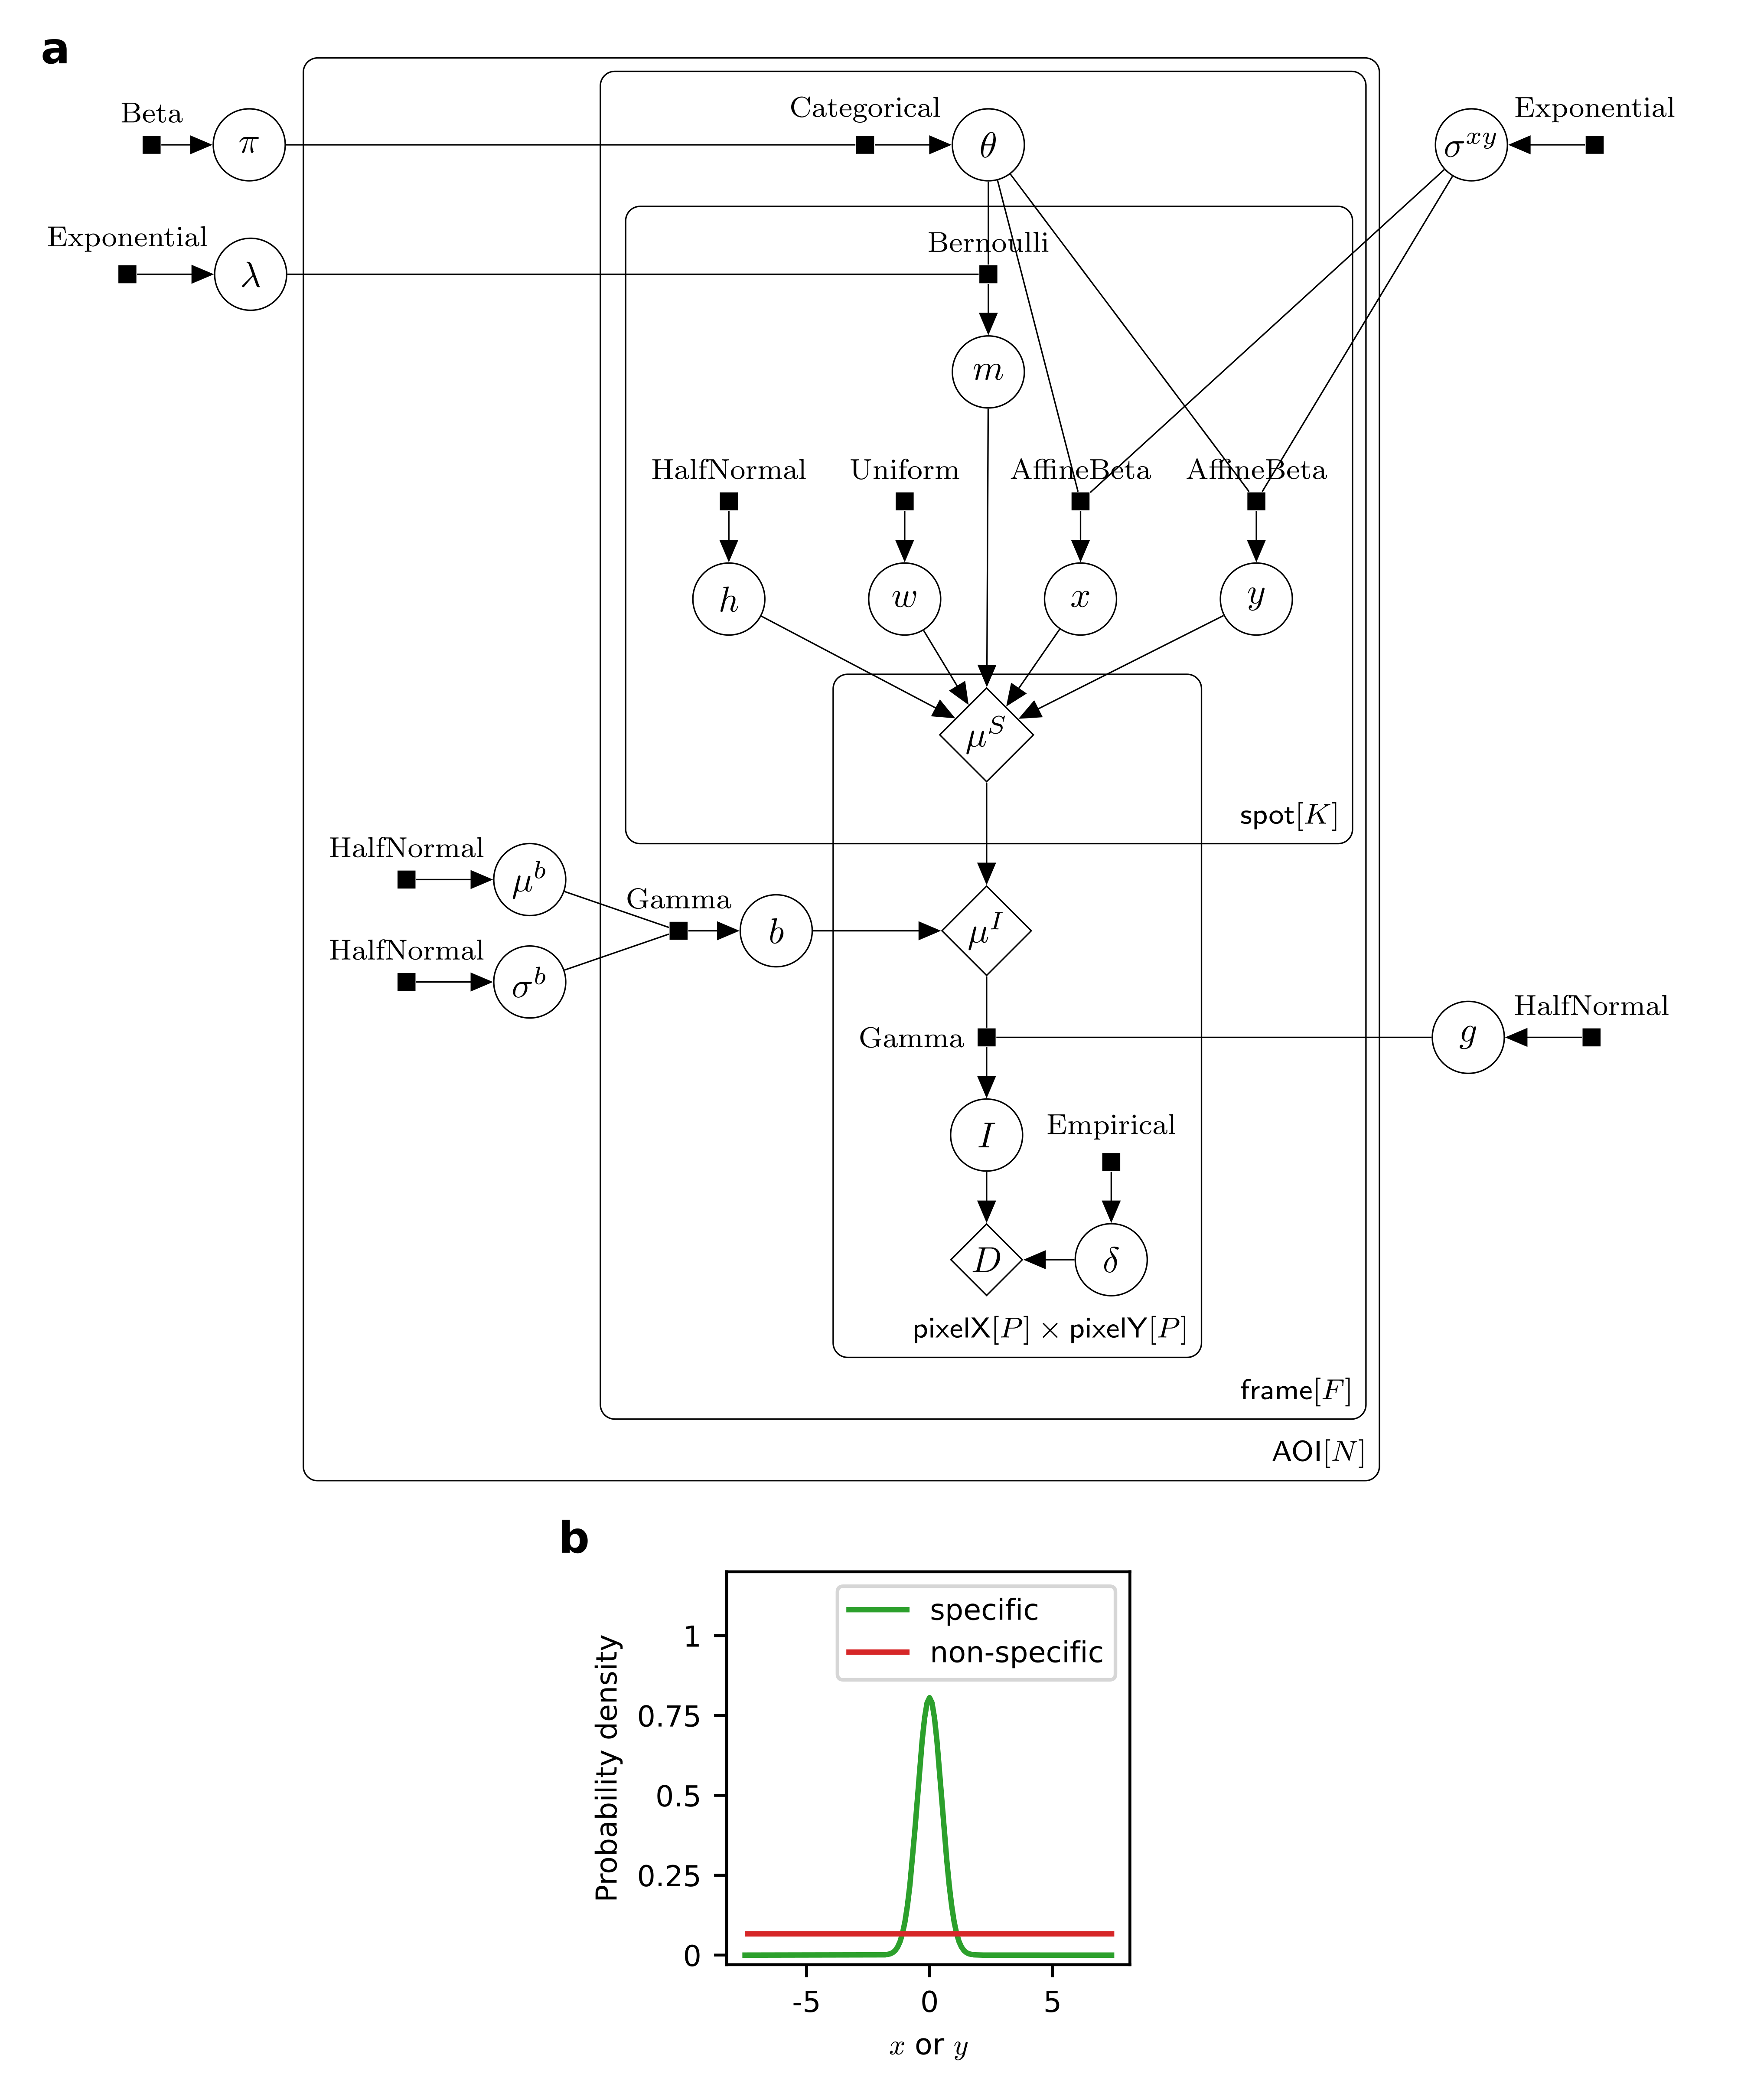
\includegraphics[width=\textwidth]{extended-data/figure1/figure1.png}
\label{fig:full_model}
\end{figure}

%\addtocounter{figure}{-1}
\begin{figure} [t]
\caption{\textbf{Extended graphical representation of the generative probabilistic model and the prior distributions for $x$ and $y$ spot position parameters.} \textbf{a}, Directed factor graph representation \cite{Bishop2006-oa} of model parameters and parameter distributions. Model parameters are depicted as circles, parameter distributions as small filled squares, and deterministic functions as diamonds. Names of the probability distributions are written next to the squares. Input parameters and output parameters are connected by lines, with an arrow pointing towards the dependent parameter. Observed image ($D$) is the sum of the noisy photon-dependent image ($I$) and the photon-independent camera offset ($\delta$). Plates (rounded rectangles) contain nodes that are repeated for the number of instances displayed at the bottom-right corner: number of AOIs ($N$), frame count ($F$), maximum number of spots in a single image ($K$), and number of image pixels ($P \times P$). \textbf{b}, Prior distributions of $x$ and $y$ for specific and non-specific binding. Probability densities for $x$ and $y$ are defined in the range $\left[ -(P+1)/2, (P+1)/2 \right] $ relative to the target molecule and are conditional on the identity of the spot (specific or non-specific).  Probability densities for $x$ and $y$ parameters are identical. }
\end{figure}
%have a row above each data set with an experiment description, align columns
\clearpage

\begin{figure}[h]
\centering
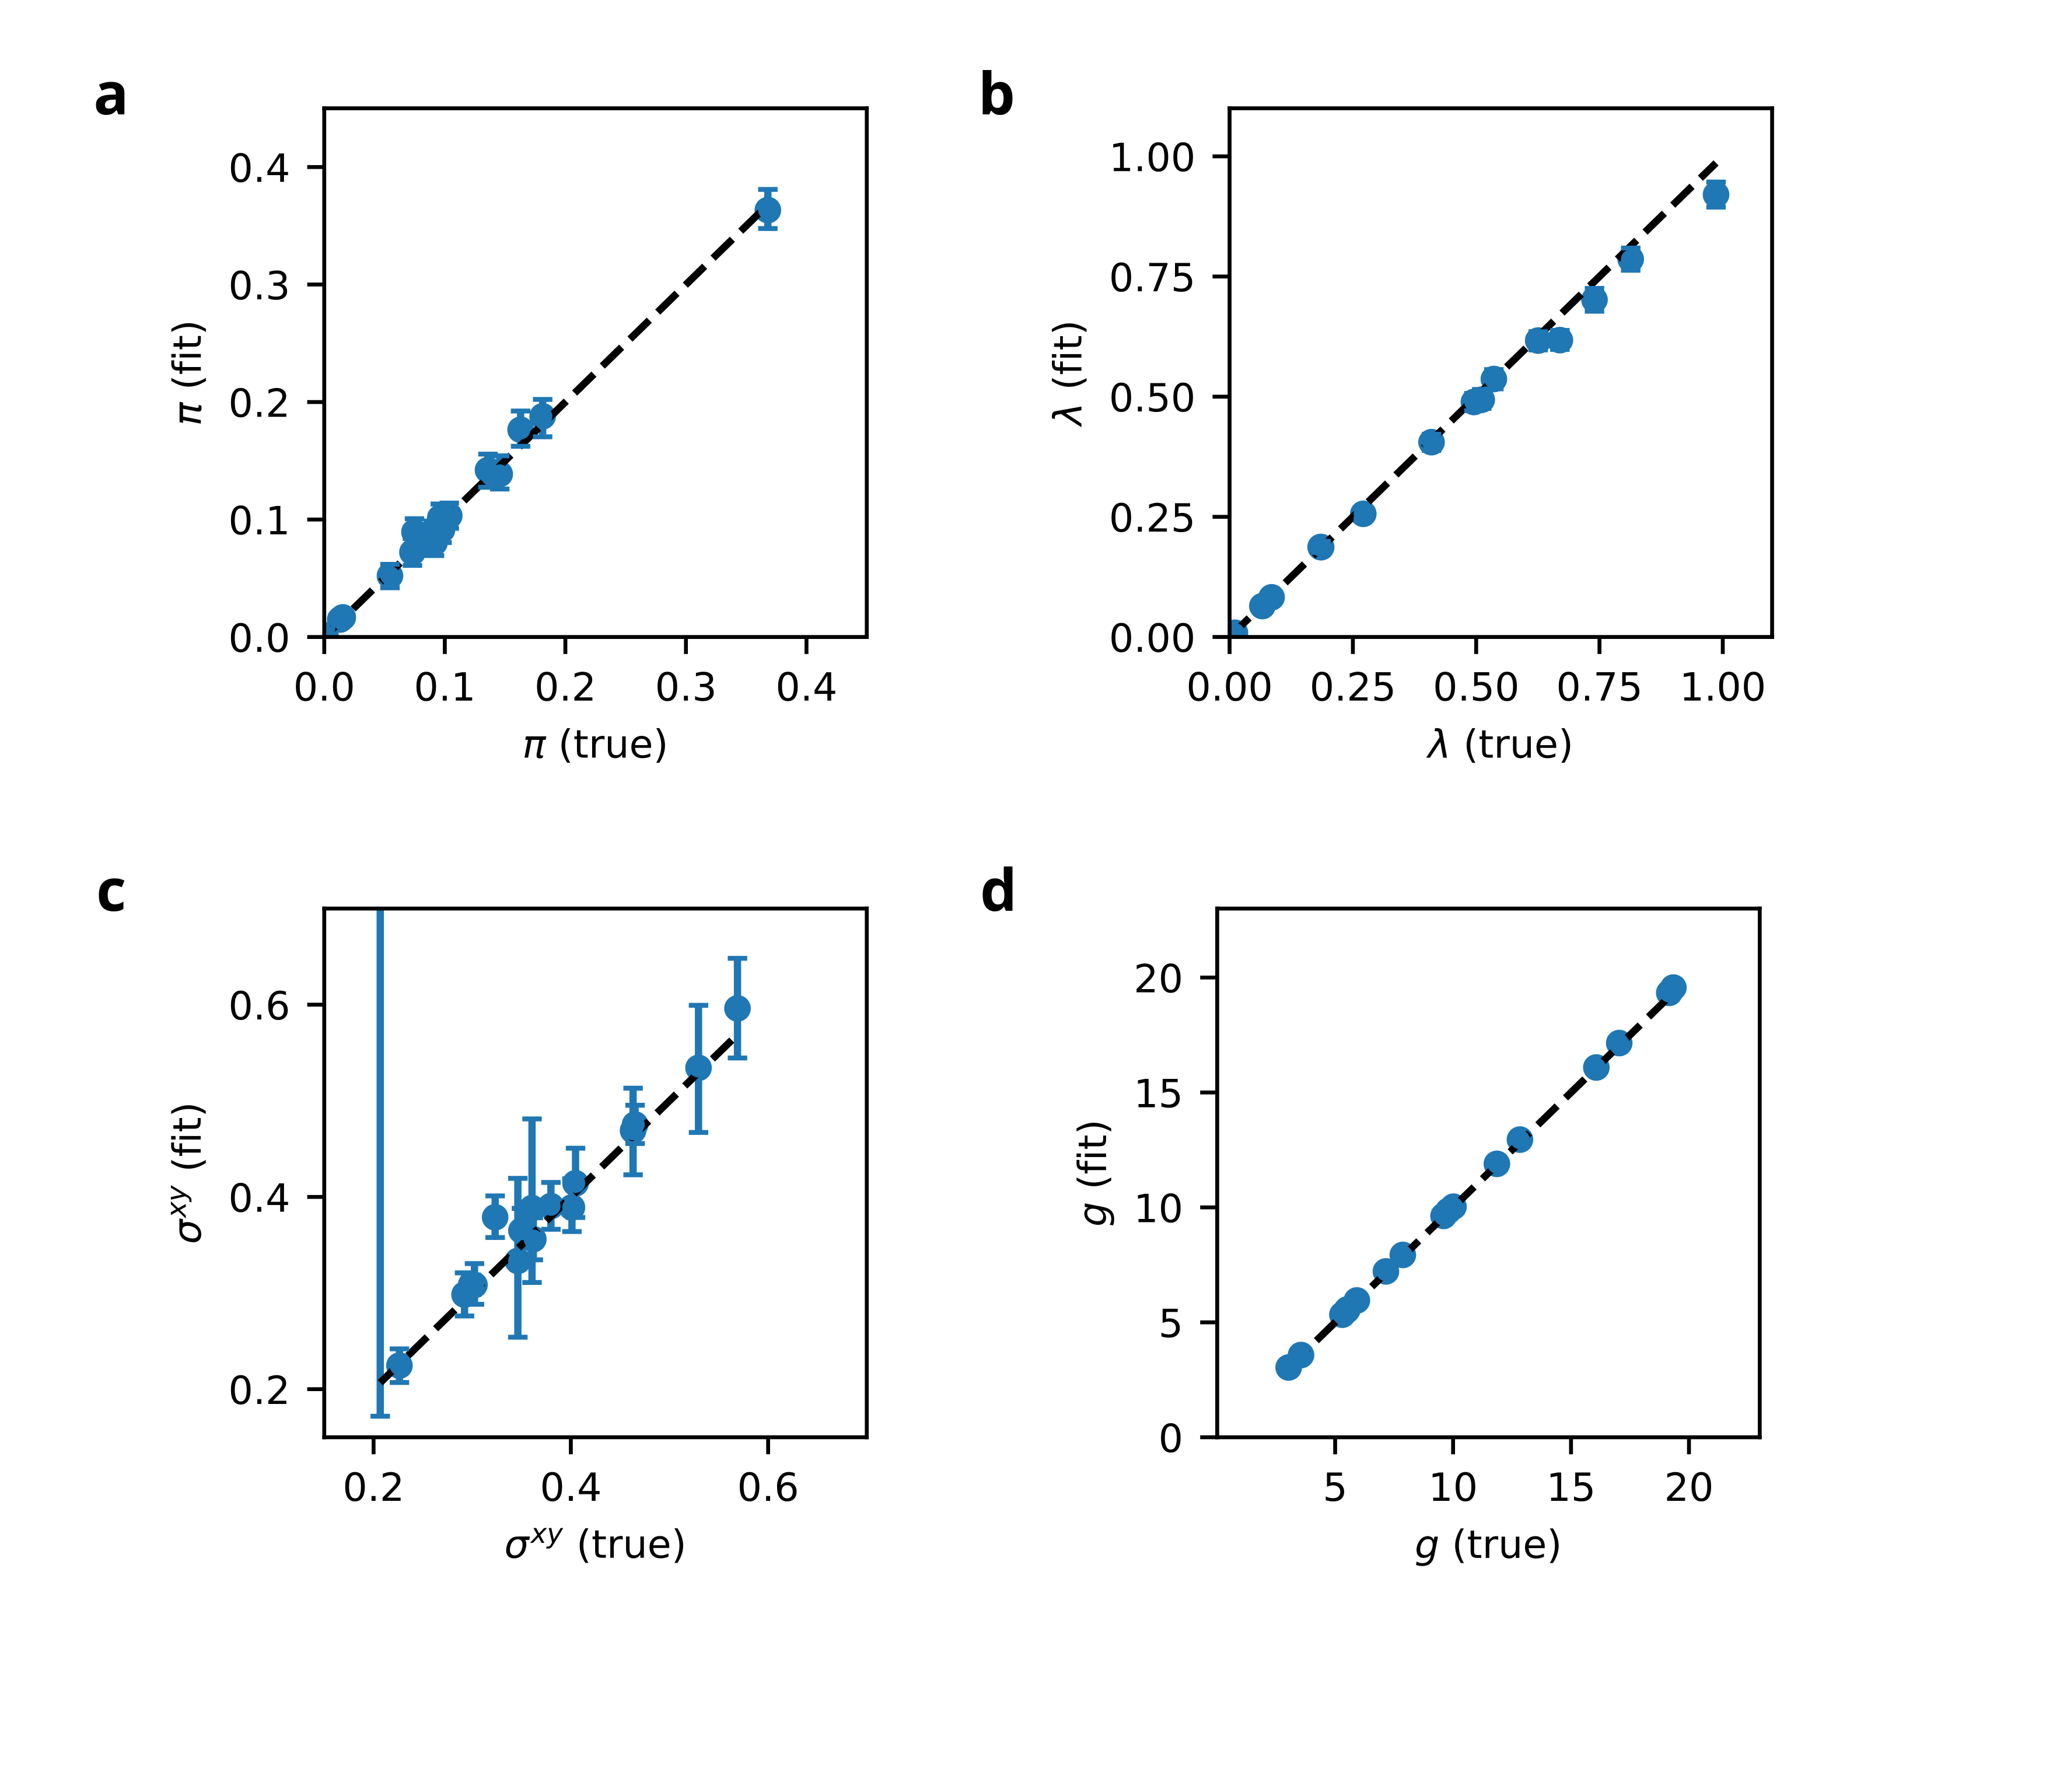
\includegraphics[width=\textwidth]{extended-data/figure2/figure2.png}
\caption{\textbf{Tapqir analysis of image data simulated using a broad range of global parameters.} Simulations }
\label{fig:tapqir_global}
\end{figure}
\pagebreak

% extended figure 3
\begin{figure}[h]
\centering
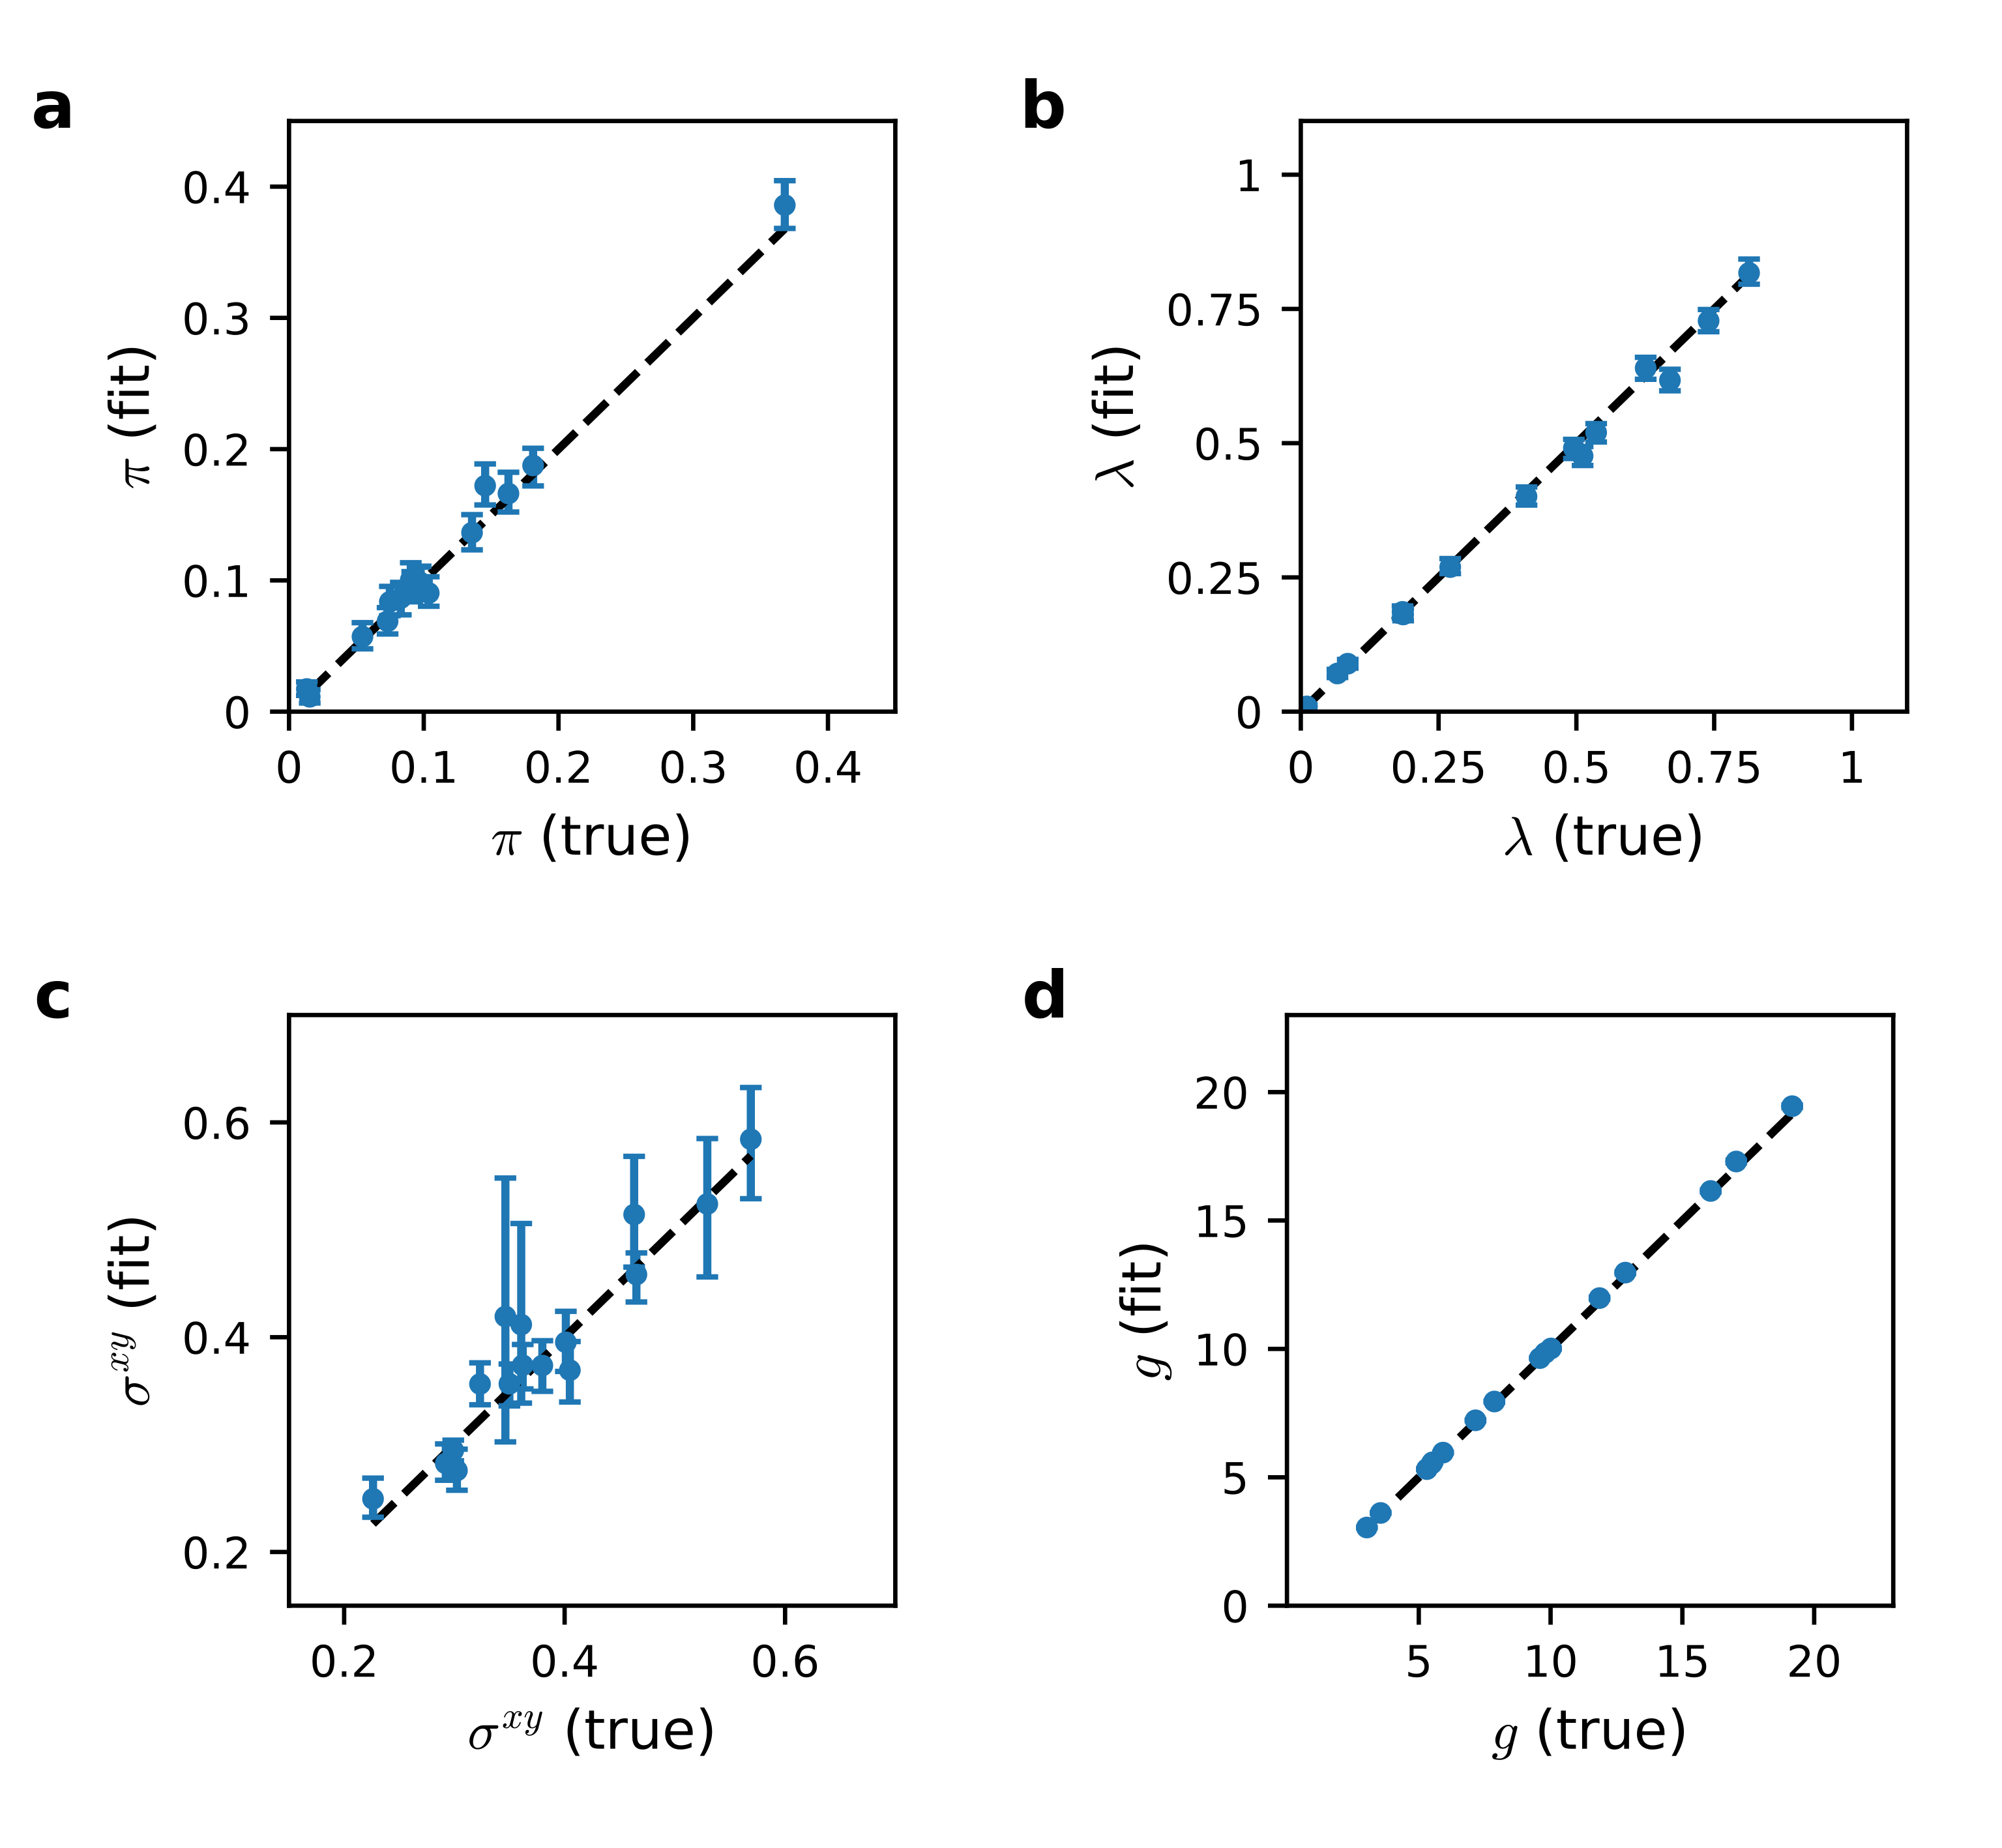
\includegraphics[width=\textwidth]{extended-data/figure3/figure2.png}
\caption{\textbf{Tapqir analysis of image data simulated using a broad range of global parameters.} Simulations (see Methods) consist of 16 datasets where values of global parameters ($\pi$, $\lambda$, $\sigma^{xy}$, and $g$) where randomly generated for each dataset (Supplementary Data 2). Simulated data were fit with Tapqir, and parameter values from the fit (with 95\% CI) are plotted against the true parameter values. To guide the eye, dashed lines  indicate identical true and fit values. \textbf{a}, Average specific binding probability $\pi$. \textbf{b}, Nonspecific binding rate $\lambda$. \textbf{c}, Proximity parameter $\sigma^{xy}$. \textbf{d}, Gain of the camera $g$. }
\label{fig:tapqir_global}
\end{figure}
\pagebreak

% extended figure 3
\begin{figure}[t]
\centering
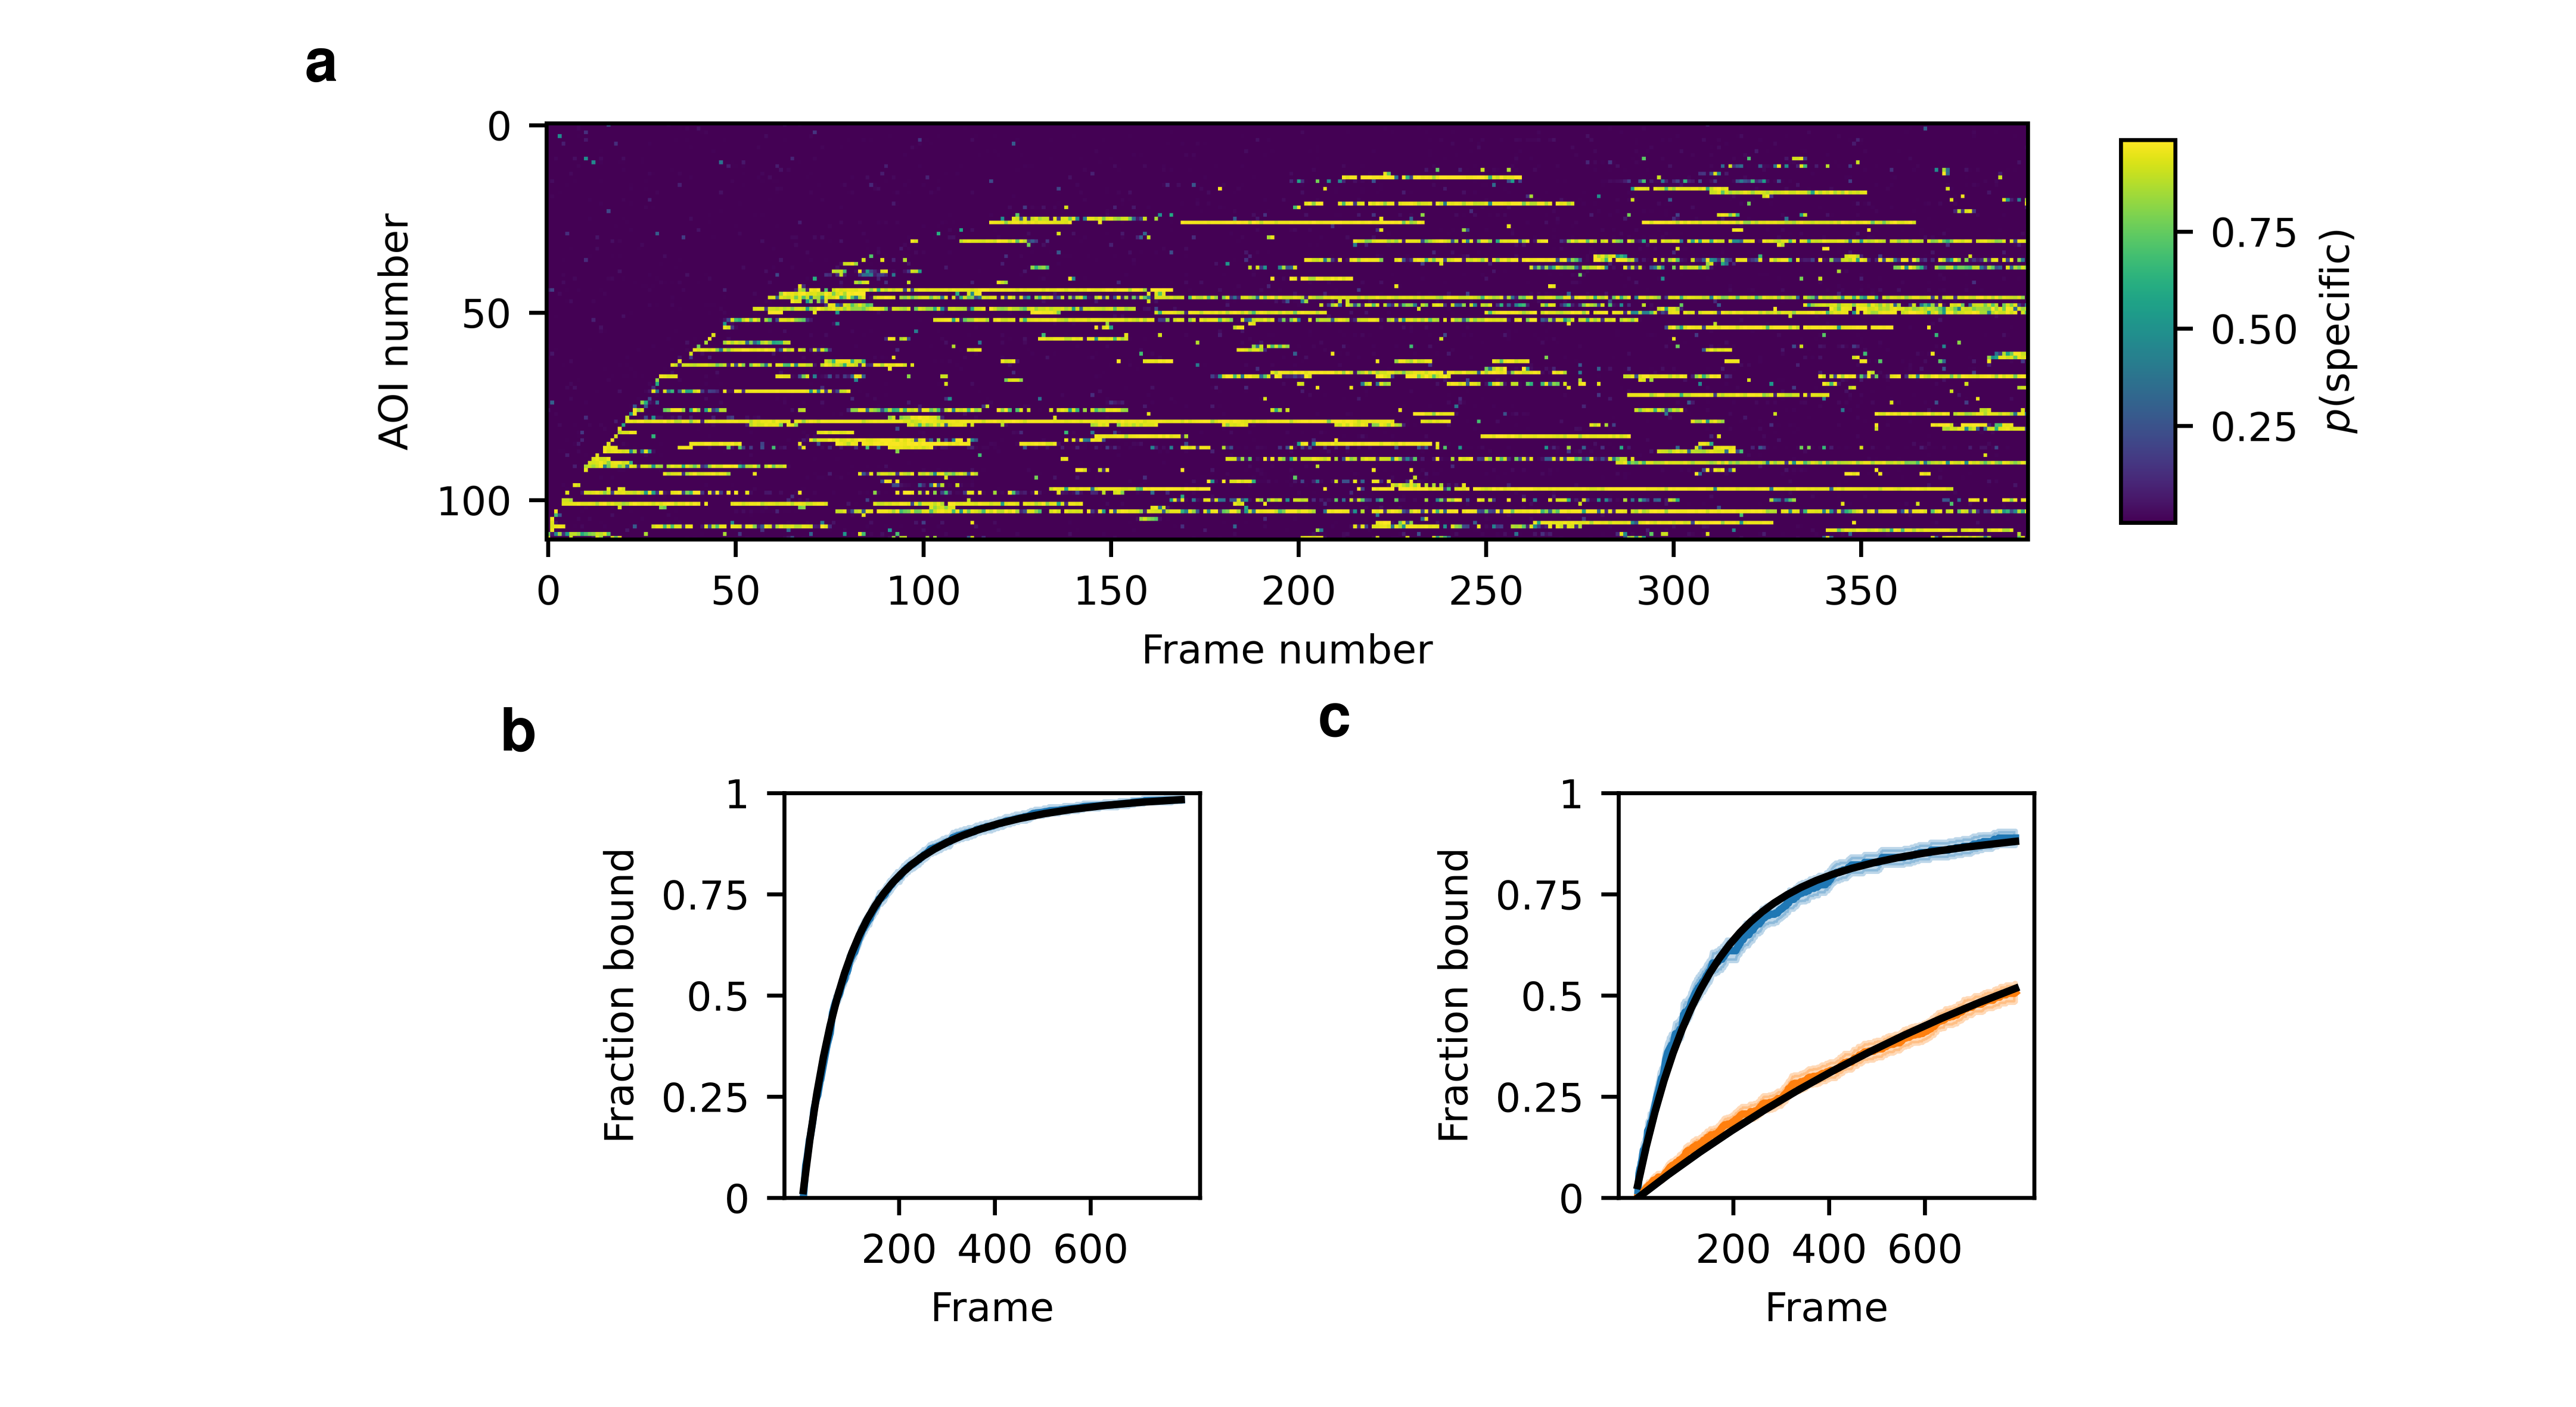
\includegraphics[width=\textwidth]{extended-data/figure4/figure3.png}
\caption{\textbf{Time-to-first binding analysis of experimental data.}  Determining association rates for experimental CoSMoS data using the time-to first binding analysis. \textbf{a}, Rastergram representation of $p(\mathsf{specific})$ (color scale) for every 3\textsuperscript{rd} AOI and every 2\textsuperscript{nd} frame of Rbp1\textsuperscript{SNAP549}-DNA\textsuperscript{488} dataset (Extended Data Table 1). DNA locations ordered by time-to-first binding. \textbf{b,c}, Determining the association rate constant for the same data set by  time-to-first-binding analysis using Tapqir (\textbf{b}: $k_\mathrm{a} = 3.56 \: [2.64, 5.37] \times 10^{-3}$ s$^{-1}$, $k_\mathrm{ns} = 1.51 \: [0.61, 2.29] \times 10^{-3}$ s$^{-1}$, $A_\mathrm{f} = 0.67 \: [0.35, 0.94]$) and an empirical spot-picker method (\textbf{c}: $k_\mathrm{a} = 2.2 \: [1.7, 2.8] \times 10^{-3}$ s$^{-1}$, $k_\mathrm{ns} = 3.1 \: [2.7, 3.5] \times 10^{-4}$ s$^{-1}$, $A_\mathrm{f} = 0.75 \: [0.66, 0.82]$) \cite{Rosen2020-zn}.   Cumulative fraction of target sites that exhibited one or more binding events by the indicated time (blue) and fit curve (black) yielding best-fit values for $k_\mathrm{a}$, $k_\mathrm{ns}$, and $A_\mathrm{f}$. Shading indicates 68\% confidence interval.
}
\label{fig:rpb1snap549}
\end{figure}
\pagebreak

% extended figure 4
\begin{figure}[t]
\centering
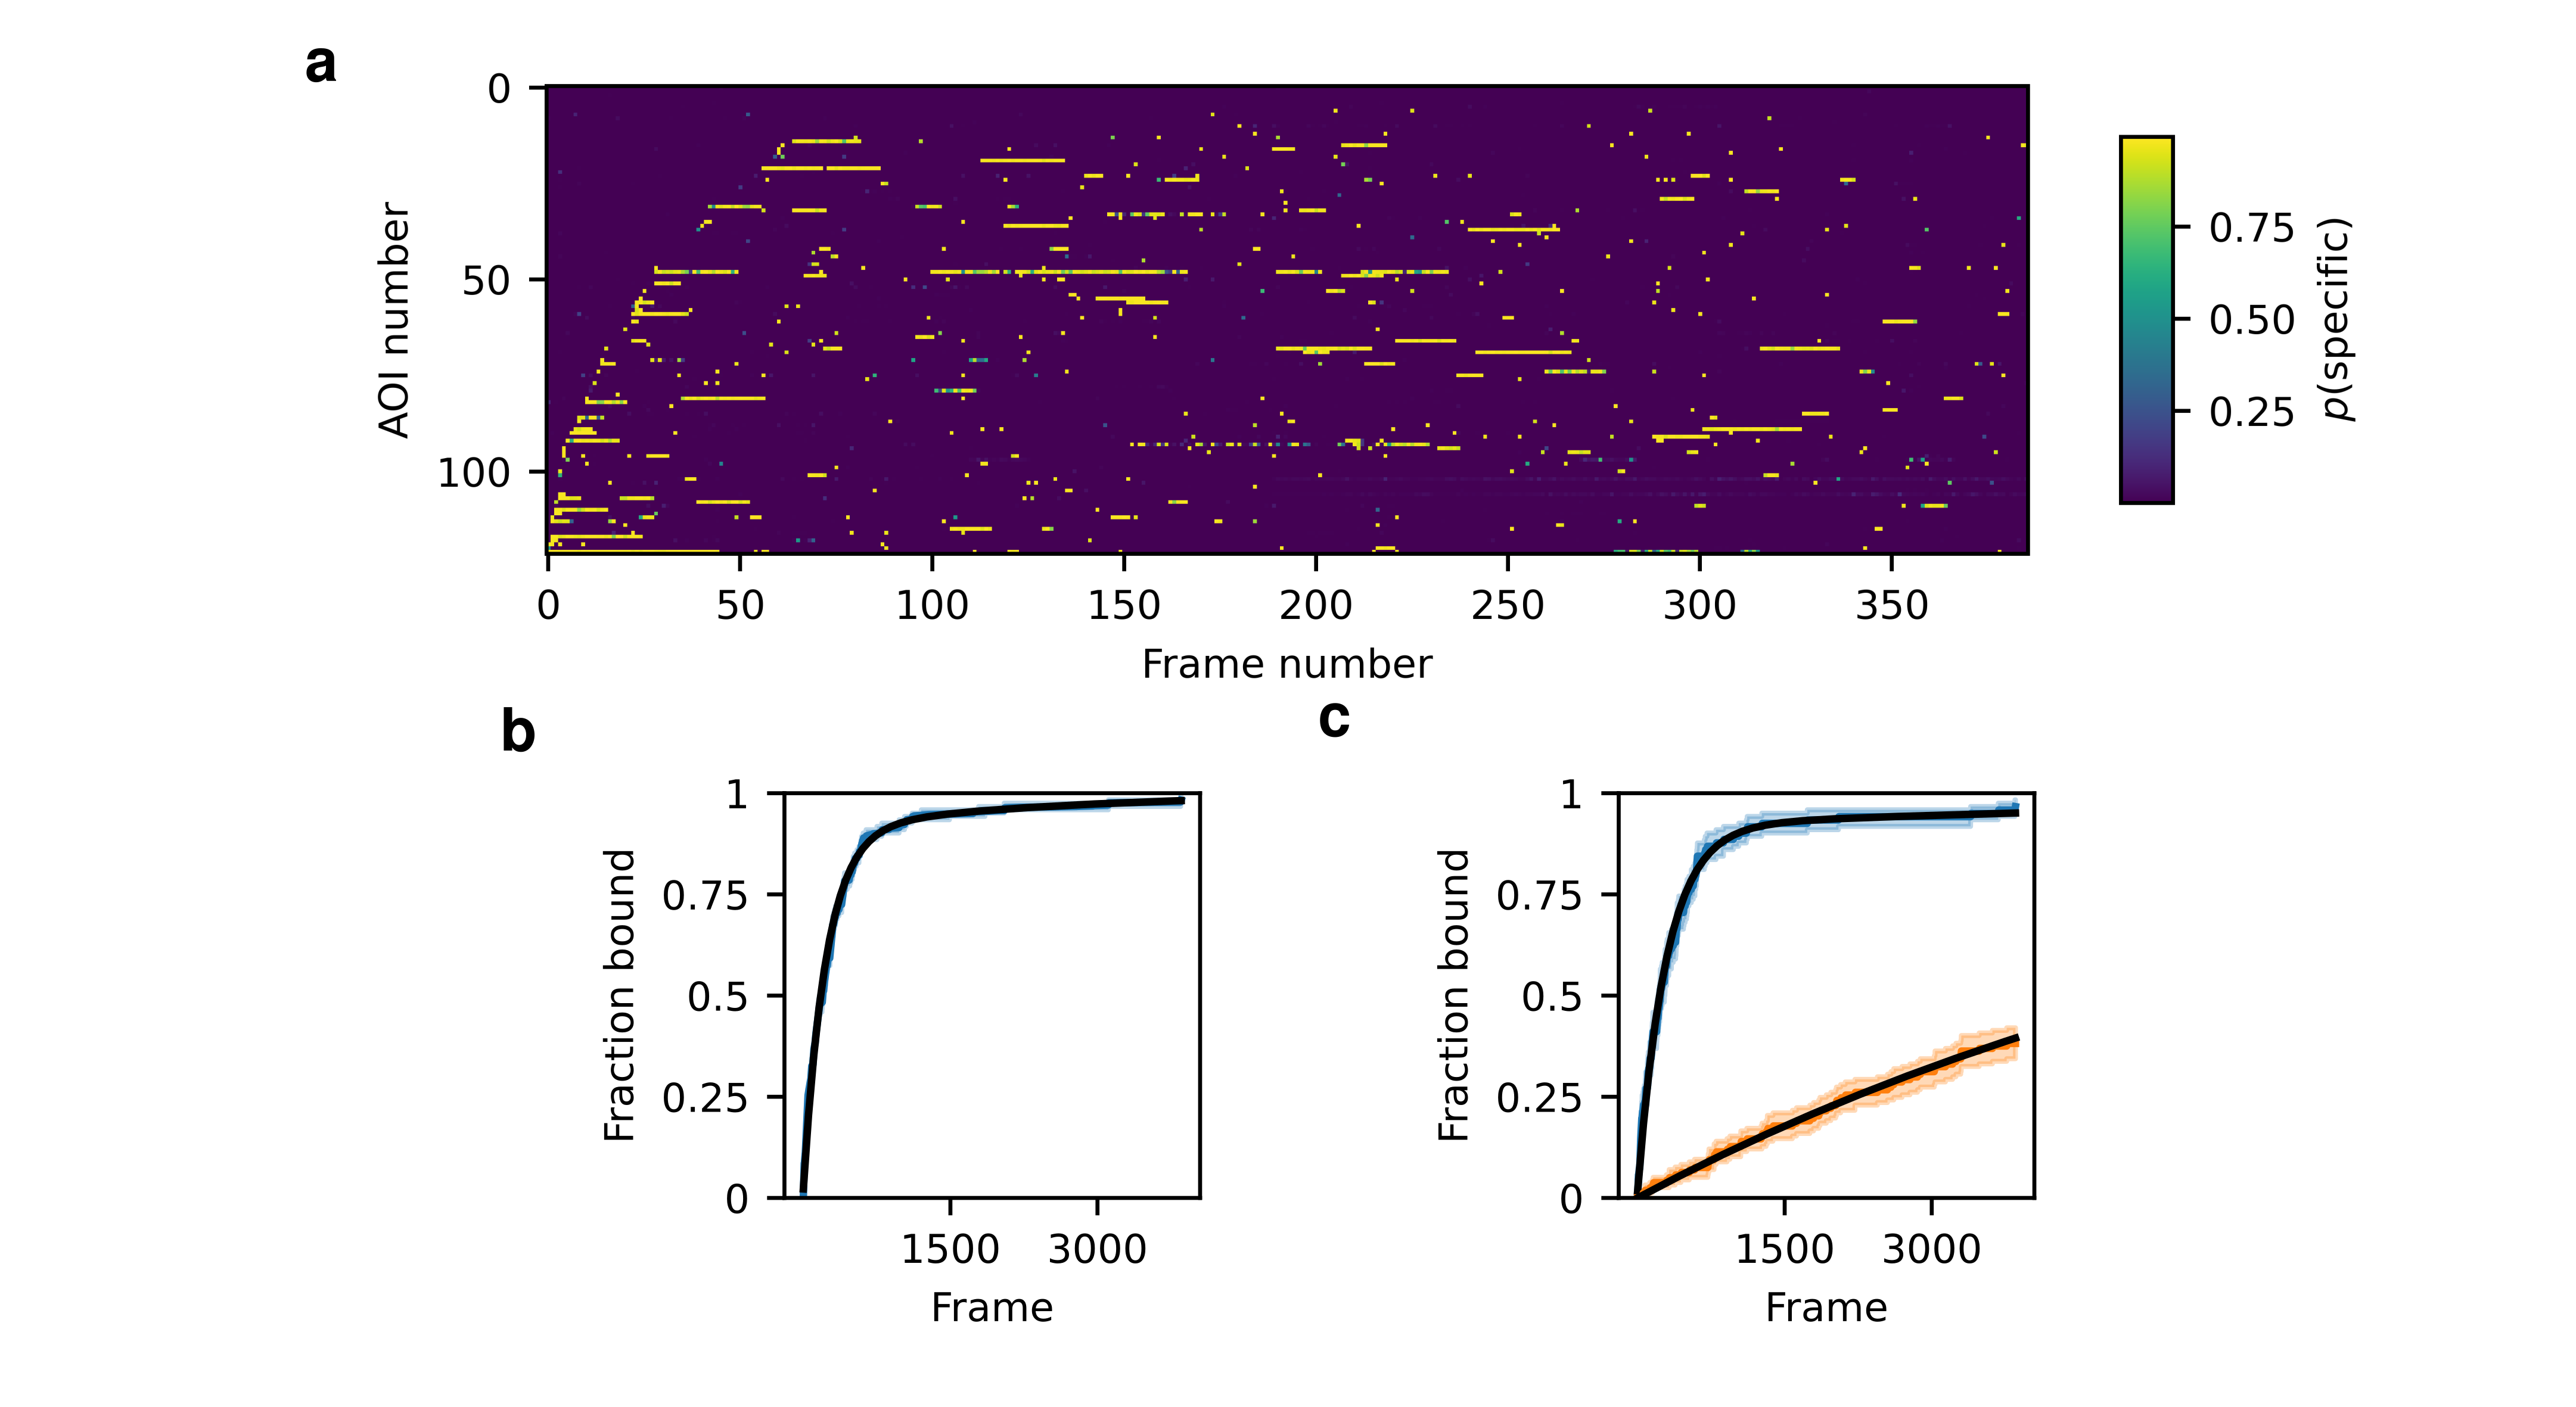
\includegraphics[width=\textwidth]{extended-data/figure5/figure4.png}
\caption{\textbf{Time-to-first binding analysis of experimental data.}  \textbf{a}, Rastergram representation of Tapqir-calculated target-specific spot  probabilities $p(\mathsf{specific})$ (color scale) for every 10\textsuperscript{th} frame of data at 122 different target locations.  AOIs were ordered by decreasing times-to-first-binding. Data set: $\sigma^{54}$RNAPCy3-598P2993 in Extended Data Table 1. \textbf{b,c}, Determining the association rate constant for the same data set by  time-to-first-binding analysis using Tapqir (\textbf{b}: $k_\mathrm{a} = 3.88 \: [3.39, 4.37] \times 10^{-3}$ s$^{-1}$, $k_\mathrm{ns} = 4.23 \: [1.77, 8.14] \times 10^{-4}$ s$^{-1}$, $A_\mathrm{f} = 0.904 \: [0.84, 0.95]$) and an empirical spot-picker method (\textbf{c}: $k_\mathrm{a} = 3.28 \: [2.64, 4.05] \times 10^{-3}$ s$^{-1}$, $k_\mathrm{ns} = 1.3 \: [1.0, 1.6] \times 10^{-4}$ s$^{-1}$, $A_\mathrm{f} = 0.92 \: [0.86, 0.97]$) \cite{Friedman2013-sf}. Cumulative fraction of target sites that exhibited one or more binding events by the indicated time (blue) and fit curve (black) yielding best-fit values for $k_\mathrm{a}$, $k_\mathrm{ns}$, and $A_\mathrm{f}$. Shading indicates 95\% confidence interval.
}
\label{fig:sigma54_298P2993}
\end{figure}
\clearpage
\pagebreak

% clean up table formatting
\begin{table}[h]
\caption{\label{tab:datasets} \textbf{Experimental datasets.}}
\resizebox{\textwidth}{!}{%
% Use "S" column identifier to align on decimal point 
\begin{tabular}{lrrrrrr}
\toprule
Dataset & size & SNR & $\pi$ & $\lambda$ & $g$ & $\sigma^{xy}$ \\
\midrule
Rpb1\textsuperscript{SNAP549}-DNA\textsuperscript{488} & \begin{tabular}[x]{@{}c@{}}$N = 331$, $F = 790$\\$N_c = 526$, $F_c = 790$\end{tabular} & $1.61$ &
$0.107$ & $0.29$ & $6.64$ & $0.56$ \\
\multicolumn{7}{l}{\footnotesize{\parbox{\textwidth}{(Single molecule experiment measuring the binding rate of Rpb1\textsuperscript{SNAP549} to DNA\textsuperscript{488} \cite{Rosen2020-zn})}}} \rule{0pt}{3ex} \\
\midrule
$\sigma^{54}$RNAPCy3-598P2993 & \begin{tabular}[x]{@{}c@{}}$N = 122$, $F = 3855$\\$N_c = 157$, $F_c = 3855$\end{tabular} & $5.24$ & $0.026$ & $0.084$ & $16.8$ & $0.33$ \\
\multicolumn{7}{l}{\footnotesize{\parbox{\textwidth}{(Single molecule experiment measuring the binding rate of $\sigma^{54}$RNAP labeled with Cy3 to 598P2993 DNA (Fig. 3D) in \cite{Friedman2013-sf})}}} \rule{0pt}{3ex} \\
\midrule
$\sigma^{54}$RNAPCy3-597P255 & \begin{tabular}[x]{@{}c@{}}$N = 102$, $F = 4407$\\$N_c = 127$, $F_c = 4407$\end{tabular} & $3.87$ & $0.087$ & $0.12$ & $12.1$ & $0.44$ \\
\multicolumn{7}{l}{\footnotesize{\parbox{\textwidth}{(Single molecule experiment measuring the binding rate of $\sigma^{54}$RNAP labeled with Cy3 to 597P255 DNA (Fig. 1E) \cite{Friedman2013-sf})}}} \rule{0pt}{3ex} \\
\bottomrule
\multicolumn{7}{l}{\footnotesize{\parbox{\textwidth}{$N$ - number of on-target AOIs, $F$ - number of frames for on-target AOIs, $N_c$ - number of control off-target AOIs, $F_c$ - number of frames for off-target AOIs.}}} \rule{0pt}{3ex} \\
\end{tabular}}
\end{table}
\clearpage
\pagebreak

%\newcommand{\specialcell}[2][c]{%
%  \begin{tabular}[#1]{@{}r@{}}#2\end{tabular}}

% \multicolumn{6}{l}{\footnotesize{\parbox{0.9\textwidth}{$^{1}$For each dataset the first row is the randomized parameter value used in the simulation and the second row gives posterior predictions of parameter values and classification accuracy statistics. Each of the four parameters $\pi$, $\lambda$, $g$, and $\sigma^{xy}$ were independently and randomly selected from a broad range that encompasses typical experimental values. $N = 5$, $F = 500$, $N_c = 5$, $F_c = 500$, $h = 3000$, $w = 1.4$, $b = 150$, $\delta = 90$}}} \\
% \multicolumn{6}{l}{\footnotesize{\parbox{0.9\textwidth}{$^2$See Methods for SNR calculation.}}}


\begin{table}[h]
\caption{\label{tab:parameters} \textbf{Glossary of mathematical symbols.}}
\begin{tabular}{l l l}
\toprule
Symbol & Description & Domain \\
\midrule
$K$ & maximum number of spots per image & $\mathbb{N}$ \\
$N$ & number of AOIs & $\mathbb{N}$ \rule{0pt}{3ex} \\
$F$ & number of frames & $\mathbb{N}$ \rule{0pt}{3ex} \\
$P$ & number of pixels & $\mathbb{N}$ \rule{0pt}{3ex} \\
$g$ & camera gain & $\mathbb{R}_{>0}$ \rule{0pt}{3ex} \\
$\sigma^{xy}$ & proximity & $(0, (P+1)/\sqrt{12})$ \rule{0pt}{3ex} \\
$\pi$ & average target-specific binding probability & [0, 1] \rule{0pt}{3ex} \\
$\lambda$ & target-nonspecific binding rate & $\mathbb{R}_{>0}$ \rule{0pt}{3ex} \\
$\mu^b$ & mean background intensity across AOI & $\mathbb{R}_{>0}^{\mathsf{AOI}[N]}$ \rule{0pt}{3ex} \\
$\sigma^b$ & standard deviation of background intensity across AOI & $\mathbb{R}_{>0}^{\mathsf{AOI}[N]}$ \rule{0pt}{3ex} \\
$b$ & background intensity & $\mathbb{R}_{>0}^{\mathsf{AOI}[N] \times \mathsf{frame}[F]}$ \rule{0pt}{3ex} \\
$\theta$ & target-specific spot index & $\{0, 1, \dots, K \}^{\mathsf{AOI}[N] \times \mathsf{frame}[F]}$ \rule{0pt}{3ex} \\
$m$ & spot presence indicator & $\{ 0, 1 \}^{\mathsf{spot}[K] \times \mathsf{AOI}[N] \times \mathsf{frame}[F]}$ \rule{0pt}{3ex} \\
$h$ & integrated spot intensity & $\mathbb{R}_{>0}^{\mathsf{spot}[K] \times \mathsf{AOI}[N] \times \mathsf{frame}[F]}$ \rule{0pt}{3ex} \\
$w$ & spot width & $[0.75, 2.25]^{\mathsf{spot}[K] \times \mathsf{AOI}[N] \times \mathsf{frame}[F]}$ \rule{0pt}{3ex} \\
$x$ & center of the spot on the $x$-axis & $\mathbb{R}^{\mathsf{spot}[K] \times \mathsf{AOI}[N] \times \mathsf{frame}[F]}$ \rule{0pt}{3ex} \\
$y$ & center of the spot on the $y$-axis & $\mathbb{R}^{\mathsf{spot}[K] \times \mathsf{AOI}[N] \times \mathsf{frame}[F]}$ \rule{0pt}{3ex} \\
$\mu^S$ & 2-D Gaussian spot & $\mathbb{R}_{>0}^{\mathsf{spot}[K] \times \mathsf{AOI}[N] \times \mathsf{frame}[F] \times \mathsf{pixelX}[P] \times \mathsf{pixelY}[P]}$ \rule{0pt}{3ex} \\
$\mu^I$ & ideal image & $\mathbb{R}_{>0}^{\mathsf{AOI}[N] \times \mathsf{frame}[F] \times \mathsf{pixelX}[P] \times \mathsf{pixelY}[P]}$ \rule{0pt}{3ex} \\
$\delta$ & offset signal & $\mathbb{R}_{>0}^{\mathsf{AOI}[N] \times \mathsf{frame}[F] \times \mathsf{pixelX}[P] \times \mathsf{pixelY}[P]}$ \rule{0pt}{3ex} \\
$I$ & observed image w/o offset & $\mathbb{R}_{>0}^{\mathsf{AOI}[N] \times \mathsf{frame}[F] \times \mathsf{pixelX}[P] \times \mathsf{pixelY}[P]}$ \rule{0pt}{3ex} \\
$D$ & observed image & $\mathbb{R}_{>0}^{\mathsf{AOI}[N] \times \mathsf{frame}[F] \times \mathsf{pixelX}[P] \times \mathsf{pixelY}[P]}$ \rule{0pt}{3ex} \\
$x^\mathsf{target}$ & target molecule position on the $x$-axis & $[P/2-1, P/2]^{\mathsf{AOI}[N] \times \mathsf{frame}[F]}$ \rule{0pt}{3ex} \\
$y^\mathsf{target}$ & target molecule position on the $y$-axis & $[P/2-1, P/2]^{\mathsf{AOI}[N] \times \mathsf{frame}[F]}$ \rule{0pt}{3ex} \\
$i$ & pixel index on the $x$-axis & $\{0, \dots, (P-1)\}^{\mathsf{pixelX}[P]}$ \rule{0pt}{3ex} \\
$j$ & pixel index on the $y$-axis & $\{0, \dots, (P-1)\}^{\mathsf{pixelX}[P]}$ \rule{0pt}{3ex} \\
$D^\mathsf{raw}$ & raw microscope images & $\mathbb{R}_{>0}^{\mathsf{frame}[F] \times \mathsf{pixelX}[H] \times \mathsf{pixelY}[W]}$ \rule{0pt}{3ex} \\
$x^{\mathsf{target}, \mathsf{raw}}$ & target molecule position in raw images on the $x$-axis & $[-0.5, H-0.5]^{\mathsf{AOI}[N] \times \mathsf{frame}[F]}$ \rule{0pt}{3ex} \\
$y^{\mathsf{target}, \mathsf{raw}}$ & target molecule position in raw images on the $y$-axis & $[-0.5, W-0.5]^{\mathsf{AOI}[N] \times \mathsf{frame}[F]}$ \rule{0pt}{3ex} \\
\bottomrule
\end{tabular}
\end{table}
\clearpage
\pagebreak

\begin{table}[h]
\caption{\label{tab:dist} \textbf{Probability distributions used in the model.}}
\begin{tabular}{l l}
\toprule
Distribution & PDF \\
\midrule
$x \sim \mathbf{AffineBeta}(\mu, \nu, a, b)$ &
    $\dfrac{y^{\alpha-1}(1-y)^{\beta-1}}{\text{B}(\alpha, \beta)}$
    where $\alpha=\dfrac{\nu (\mu-a)}{b-a}$, $\beta=\dfrac{\nu (b-\mu)}{b-a}$, and $y = \dfrac{x-a}{b-a}$ \\
$x \sim \mathbf{Bernoulli}(\pi)$ &
    $\pi^x (1-\pi)^{1-x}$ \\
$x \sim \mathbf{Beta}(\alpha, \beta)$ &
    $\dfrac{x^{\alpha-1}(1-x)^{\beta-1}}{\text{B}(\alpha, \beta)}$ \\
$x \sim \mathbf{Categorical}_{\{z_i\}^k_{i=1}}(\mathbf{p})$ &
    $\prod_{i=1}^k p_i^{[x=z_i]}$ \\
$x \sim \mathbf{Gamma}(\mu, \sigma)$ &
    $\dfrac{\beta^\alpha}{\Gamma(\alpha)}x^{\alpha-1} e^{-\beta x}$
    where $\alpha = \dfrac{\mu^2}{\sigma^2}$ and $\beta = \dfrac{\mu}{\sigma^2}$ \\
$x \sim \mathbf{HalfNormal}(\sigma)$ &
    $\dfrac{\sqrt{2}}{\sigma \sqrt{\pi}} \exp \left( -\dfrac{x^2}{2\sigma^2} \right)$
    for  $x > 0$ \\
$k \sim \mathbf{TruncatedPoisson}(\lambda, K) $ & $ \begin{cases} 1 - e^{-\lambda} \sum_{i=0}^{K-1} \dfrac{\lambda^i}{i!} & \textrm{if $k = K$} \\ \dfrac{\lambda^k e^{-\lambda}}{k!} & \textrm{otherwise} \end{cases} $ \\
$x \sim \mathbf{Uniform}(a, b)$ &
    $\dfrac{1}{b-a}$ for $x \in [a, b]$ \\
\bottomrule
\end{tabular}
\end{table}